\chapter{Experiments and results}
\label{AER}

\section{What Does A Good Curve Look Like?}
Assuming a very simple model, with no washin or washout rate, a good bacteria growth curve would look like a mountain. 
For a given initial condition, the bacteria start to consume resources and replicate leading to exponential growth. 
The phages start to infect the bacteria and eventually the bacteria start to die. 
A clear peak with the bacteria should be noticed. 
\Cref{fig:created:a_good_curve_linear} shows an example of a good curve. 
\Cref{fig:created:a_good_curve_logarithmic} is the same plot but with a logarithmic y-axis. 

\begin{figure}[h!]
    \centering
    \begin{subfigure}{1\linewidth}
        \centering
        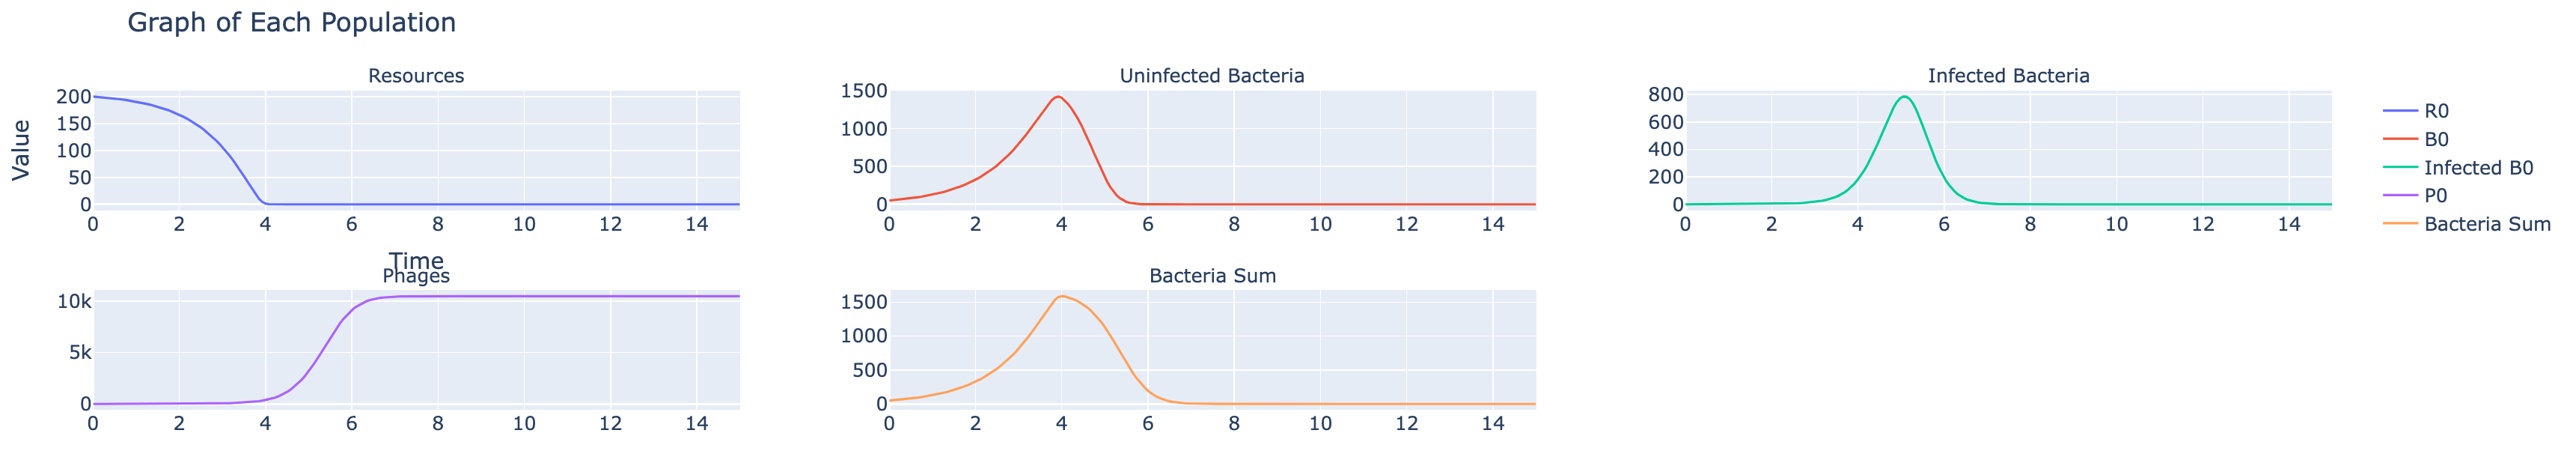
\includegraphics[width=\linewidth]{Plots/Created/a_good_plot_linear.png}
        \caption{
            Linear y-axis for a "good" plot. 
        }
        \label{fig:created:a_good_curve_linear}
    \end{subfigure}
    \hfill
    \begin{subfigure}{1\linewidth}
        \centering
        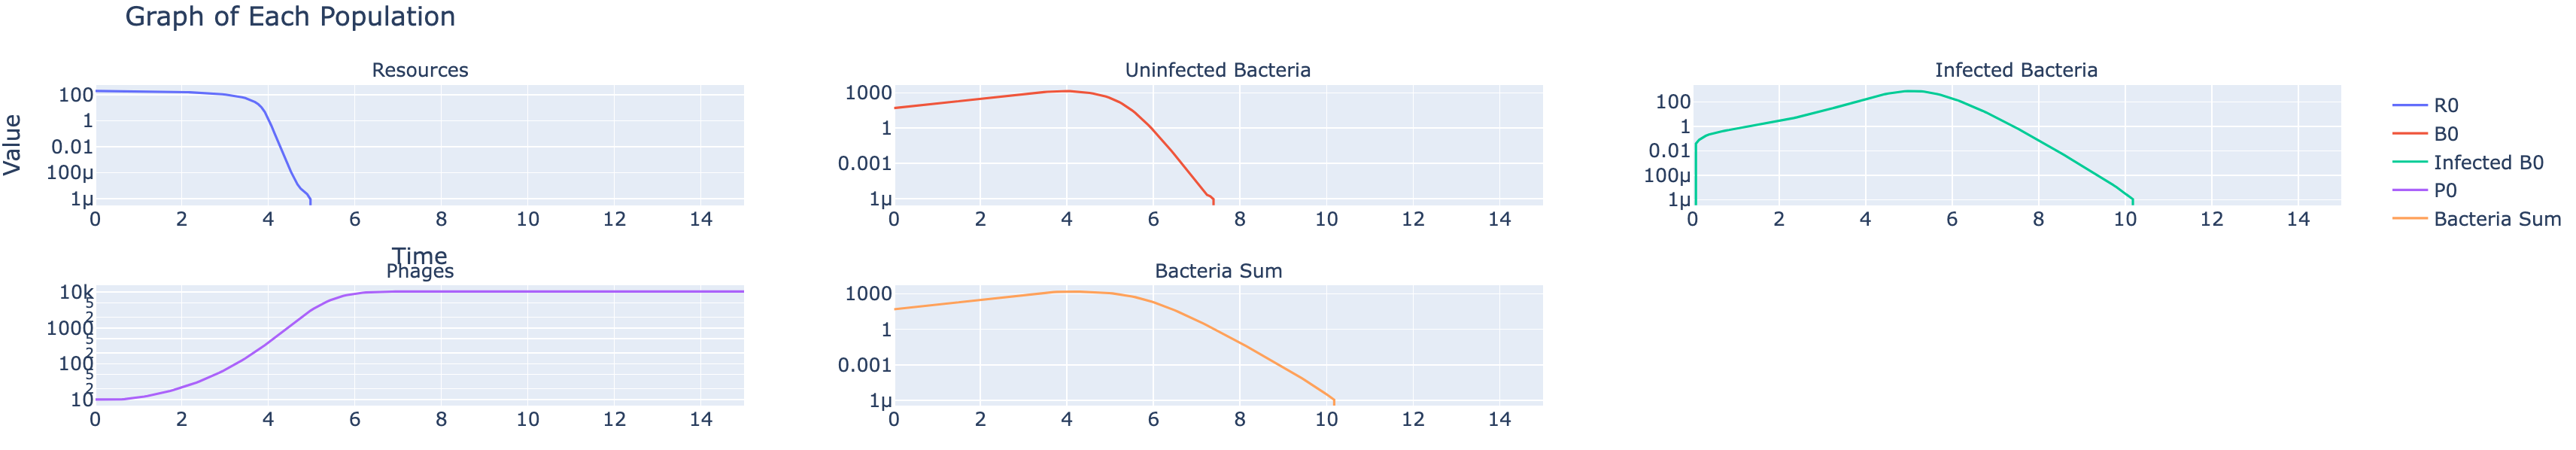
\includegraphics[width=\linewidth]{Plots/Created/a_good_plot_logarithmic.png}
        \caption{
            Logarithmic y-axis for a "good" plot. 
        }
        \label{fig:created:a_good_curve_logarithmic}
    \end{subfigure}
    \caption{
        This is what a "good" growth curve looks like. 
        As the bacteria population grows, the resource consumption speeds up until there are no resources remaining. 
        The uninfected and infected bacteria exhibit an exponential increase in growth until the phages start to infect the bacteria at around $t=4$. 
        At $t=4$ there is a noticeable increase in bacteria infections, coinciding with the peak in uninfected bacteria population at $t=4$. 
        Notice the peak in infected bacteria is at around $t=4.5$ due to the latent period infection rate. 
        The uninfected bacteria started at population of 50, and grew to a max of 1,423 at $t=3.91$. 
        The infected bacteria started at 0 and reached a peak at 784 at $t=5.05$
        The bacteria sum do not have as stark of a peak in comparison to the uninfected and infected bacteria, due to the graph measuring all bacteria populations, but the peak of 1588 at $t=3.99$ is still noticeable. 
        The phages saw an increase in population count from 10 to a maximum of 10464, a 1000x increase. 
    }
\end{figure}



\section{SOBOL Sensitivity Analysis}
\begin{figure}[h!]
    \centering
    \begin{subfigure}{0.49\linewidth}
        \centering
        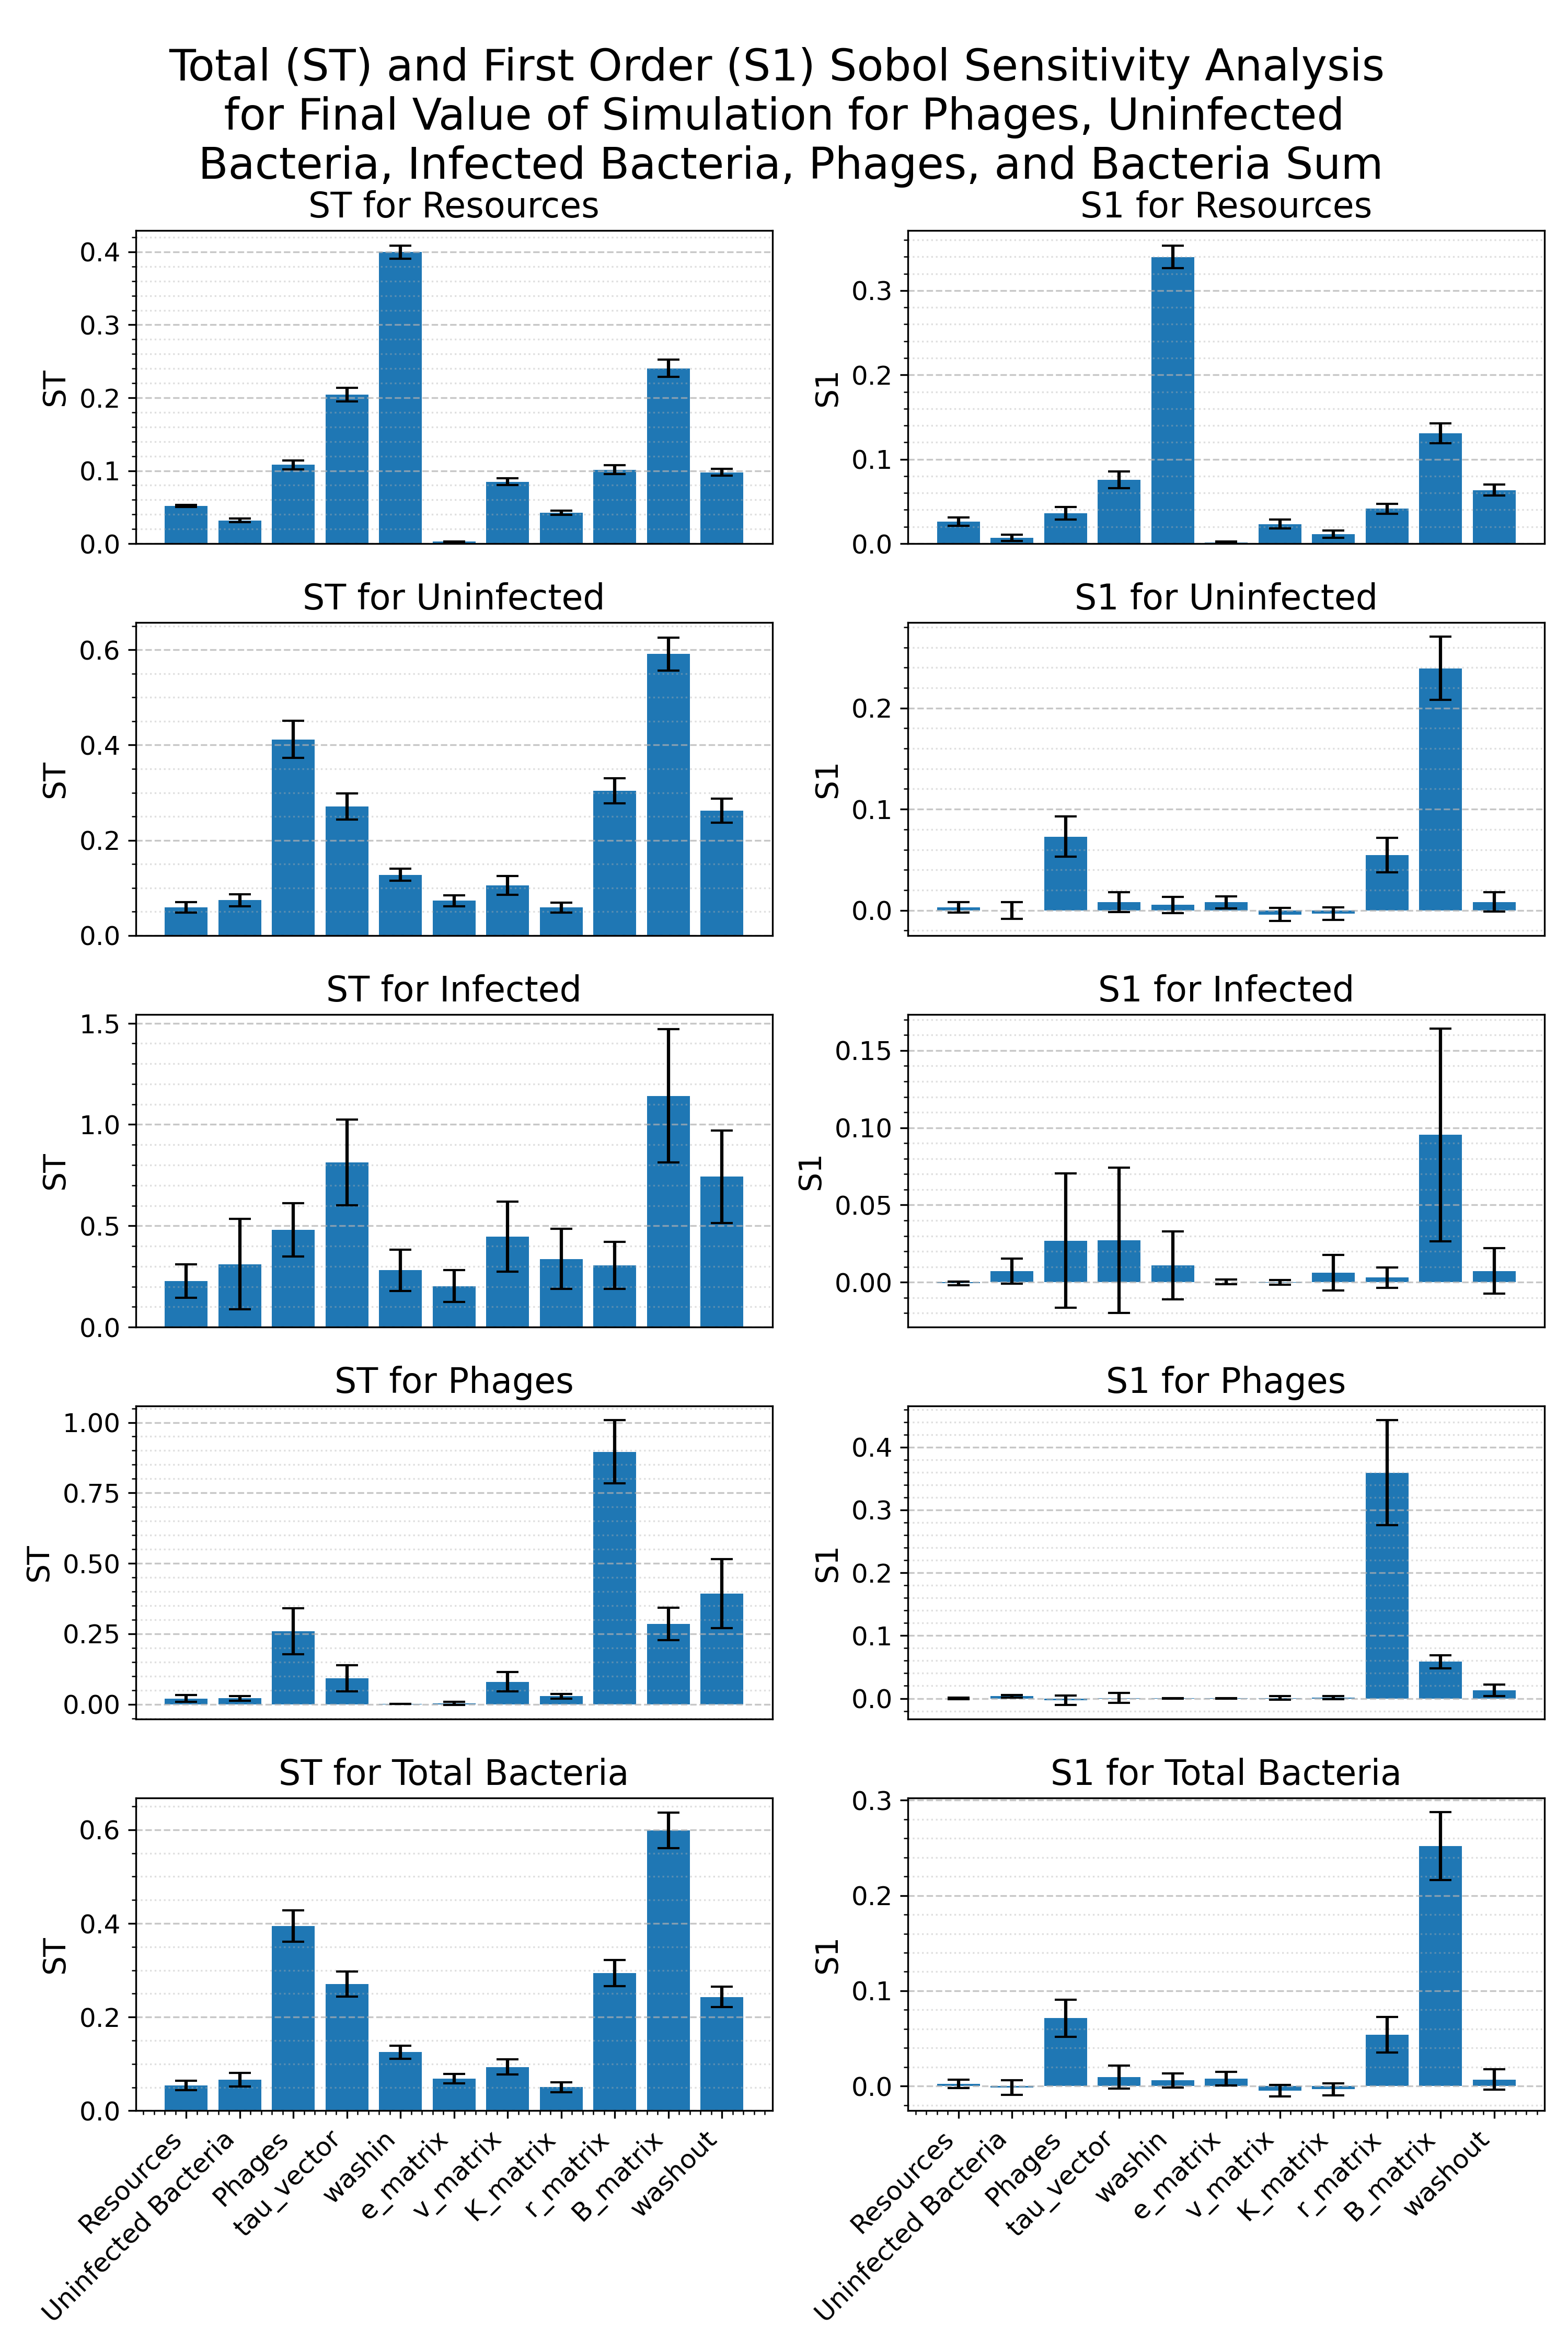
\includegraphics[width=\linewidth]{Plots/Created/SOBOL_analysis_1747923579_Final.png}
        \caption{
            The total and first order sensitivity for the golden model for the final Resource, Uninfected, Infected, Phage, and Total Bacteria population value. 
        }
        \label{fig:created:SOBOL_final}
    \end{subfigure}
    \hfill
    \begin{subfigure}{0.49\linewidth}
        \centering
        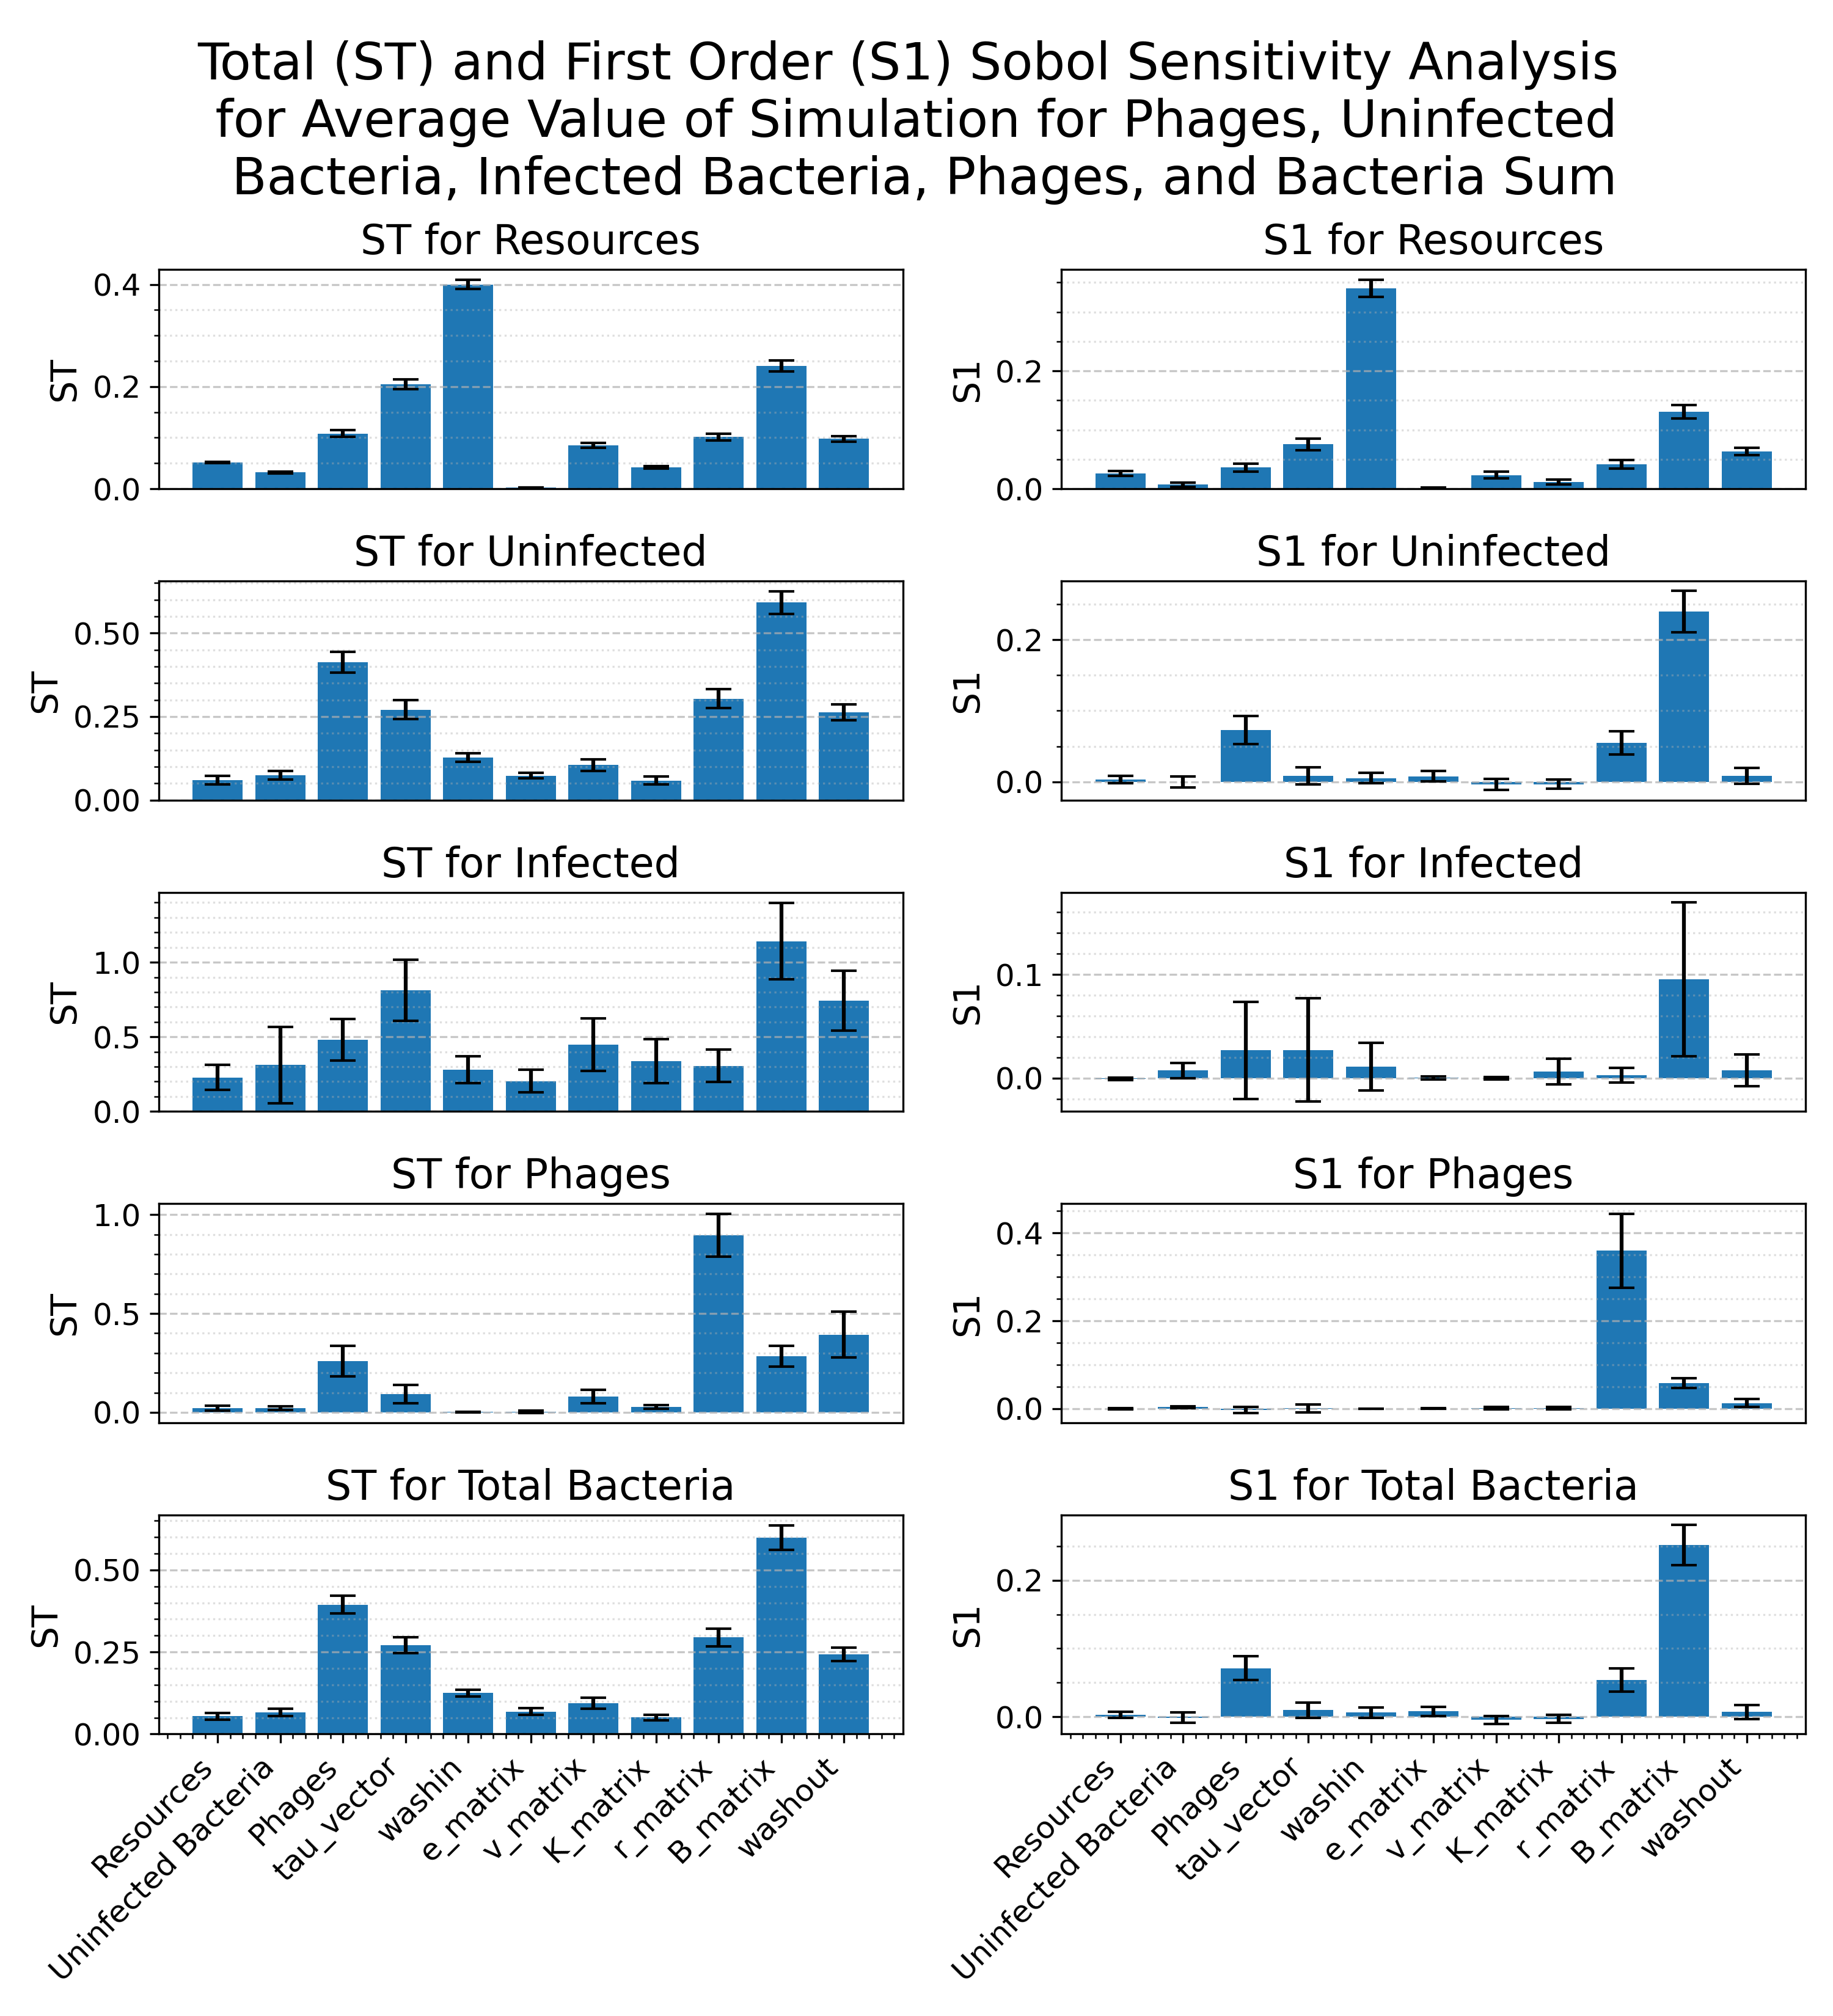
\includegraphics[width=\linewidth]{Plots/Created/SOBOL_analysis_1747923579_Average.png}
        \caption{
            The total and first order sensitivity for the golden model for the average Resource, Uninfected, Infected, Phage, and Total Bacteria population value. 
        }
        \label{fig:created:SOBOL_average}
    \end{subfigure}
    \hfill
    \begin{subfigure}{0.49\linewidth}
        \centering
        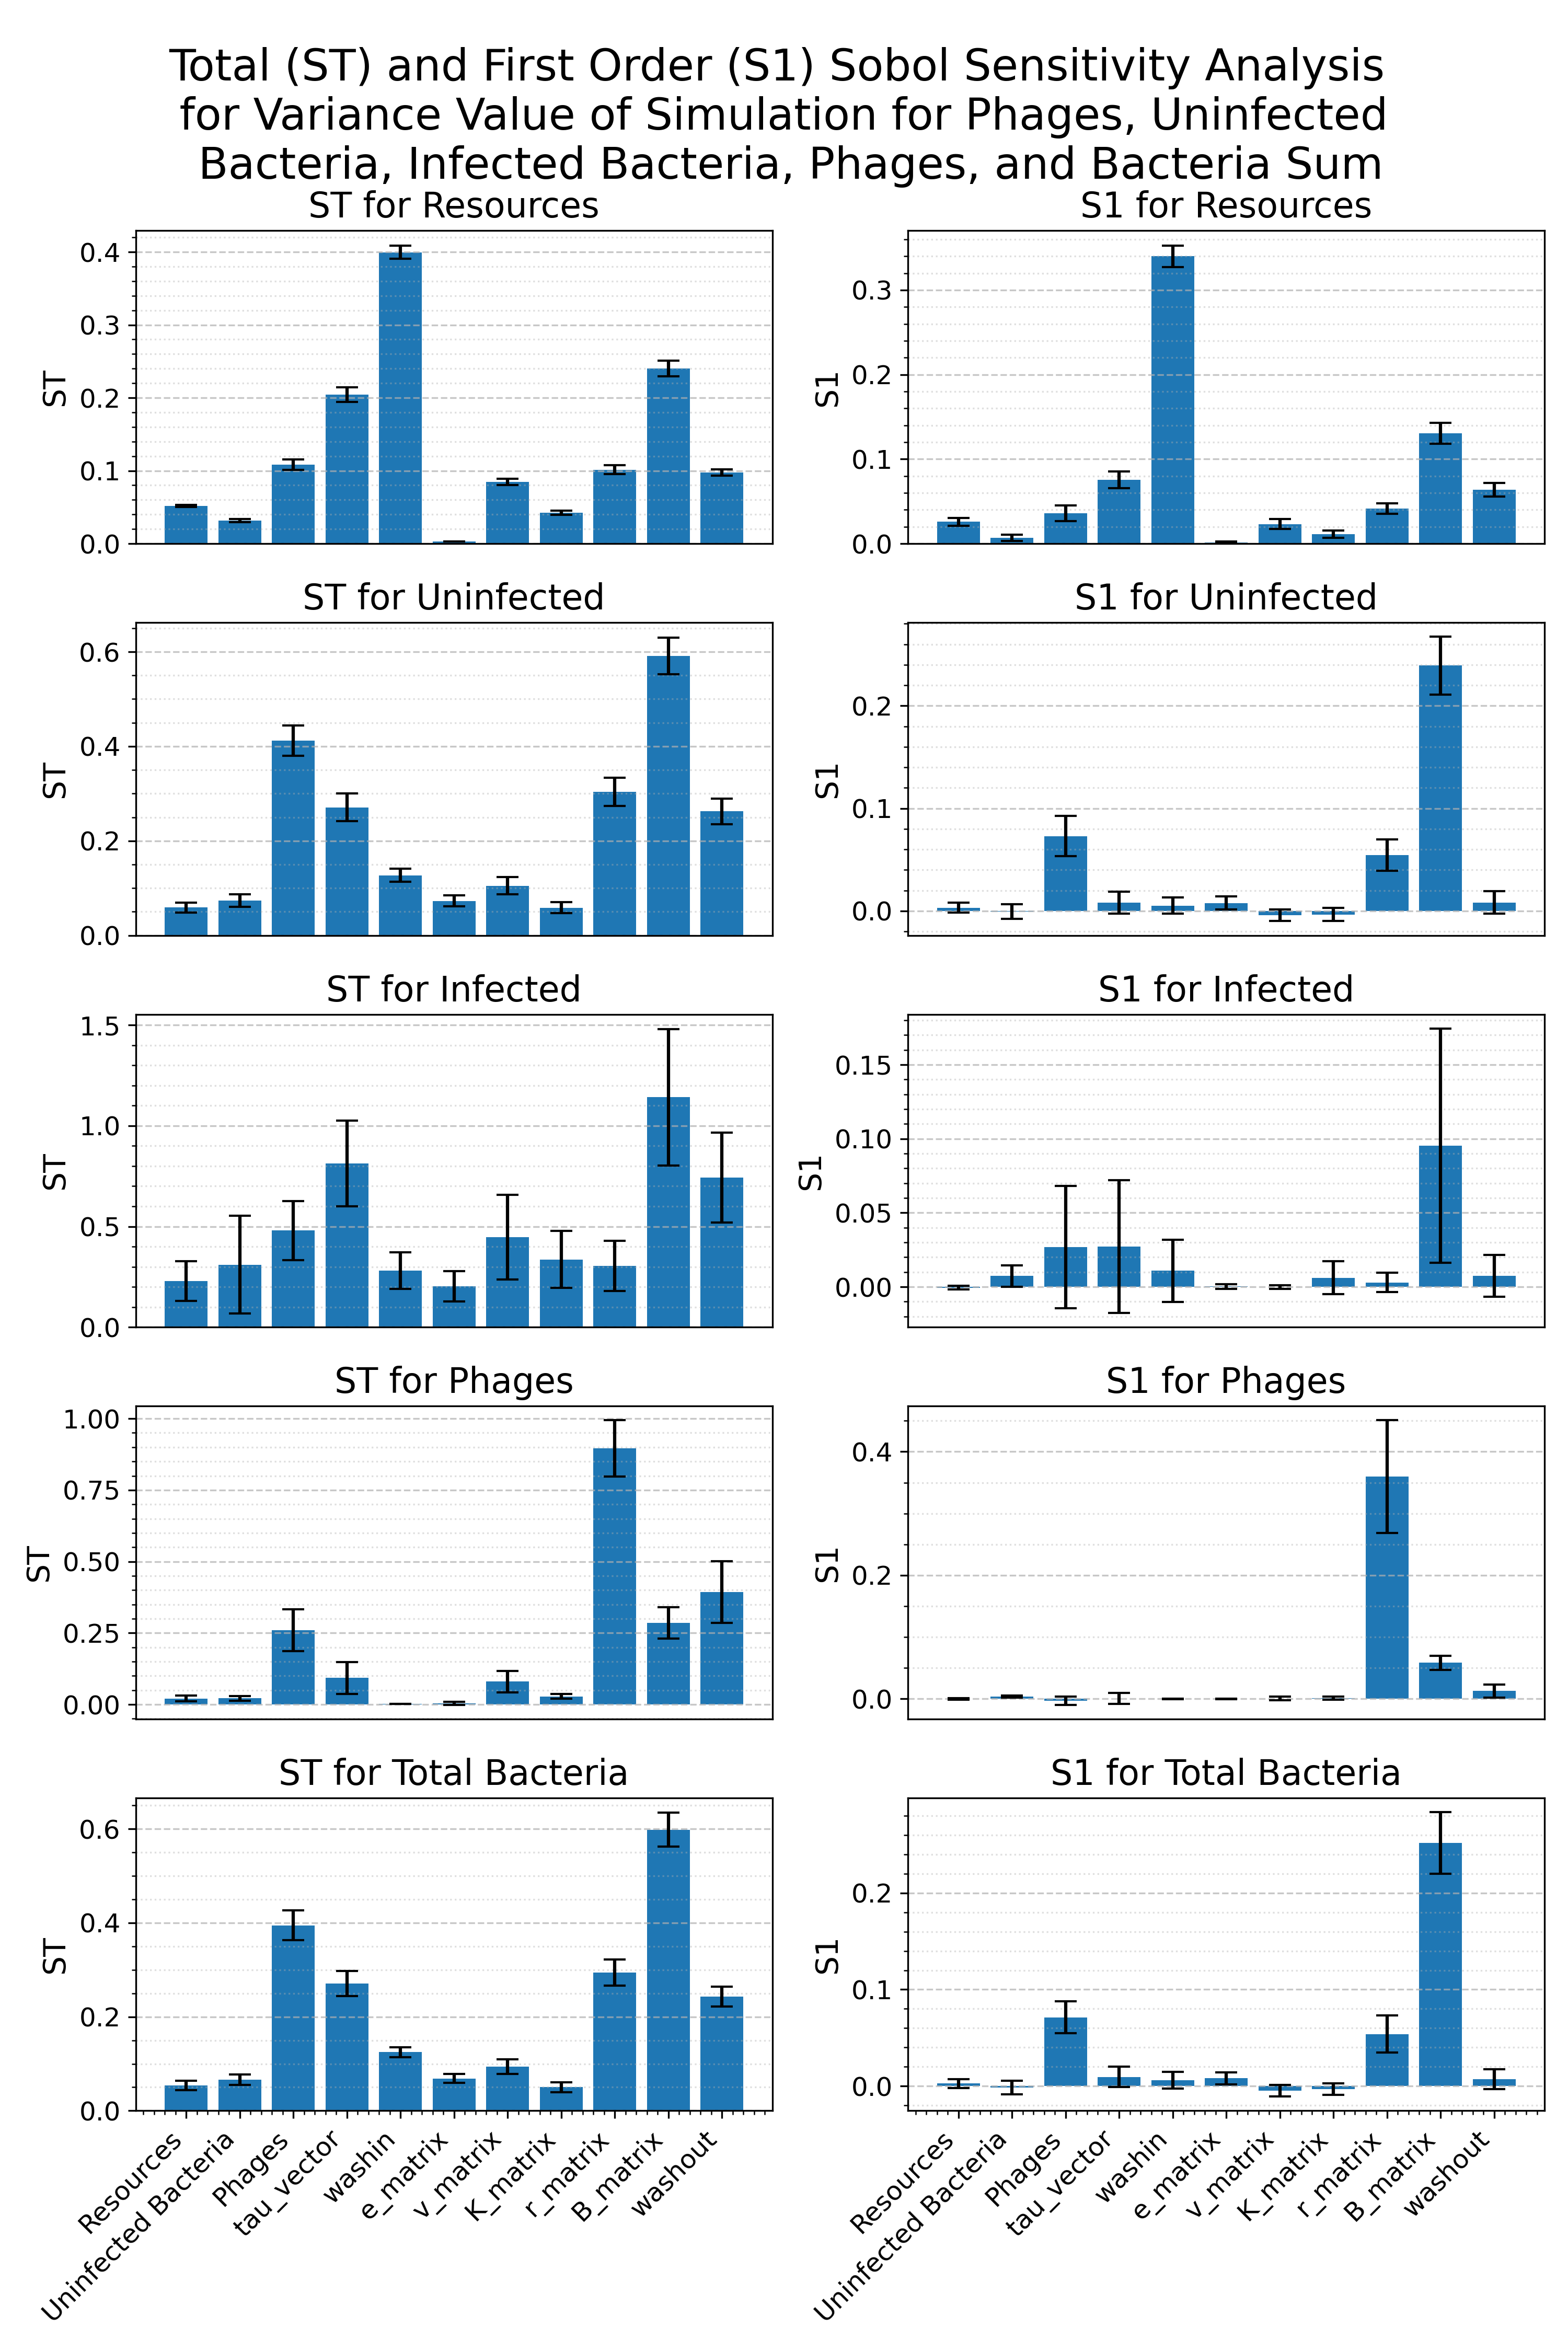
\includegraphics[width=\linewidth]{Plots/Created/SOBOL_analysis_1747923579_Variance.png}
        \caption{
            The total and first order sensitivity for the golden model for the variance of Resource, Uninfected, Infected, Phage, and Total Bacteria value. 
        }
        \label{fig:created:SOBOL_variance}
    \end{subfigure}
    \caption{The SOBOL analysis for the simple $1\times 1 \times 1$ golden model. }
\end{figure}
